\documentclass{report}
\usepackage{hyperref}
\usepackage{listings}
\usepackage{graphicx}
\usepackage[affil-it]{authblk}
\usepackage[usenames,dvipsnames]{color}
\usepackage{float}
\usepackage{wrapfig}

\usepackage{tikz}
\usepackage[bottom]{footmisc}

\usepackage{pifont}
\usepackage{tcolorbox}
\usepackage{tabularx}
\usepackage{array}
\usepackage{colortbl}
\tcbuselibrary{skins}

\title{Solution To The Expression Problem With SugarJ}
\author{
%\begin{tabular}{r@{ }l}
\bfseries Author \\
\mdseries Dominik Peuscher \\[1ex]
\bfseries Supervisors \\
\mdseries  Prof. Df. K. Ostermann\\
              Tillmann Rendel, MSc.
%\end{tabular}
}
\date{2014}
\affil{Fachbereich f\"ur Mathematik, Wirtschaftsmathematik und Informatik\\ Universit\"at Marburg}

\newcommand{\Hiline}{\makebox[0pt][l]{\color[rgb]{1,0.96,0.98}\rule[-4pt]{\linewidth}{12.5pt}}}

\newcommand{\Hilinered}{\makebox[0pt][l]{\color[rgb]{1,0.96,0.96}\rule[-4pt]{\linewidth}{12.5pt}}}
\newcommand{\Hilineyellow}{\makebox[0pt][l]{\color[rgb]{1,1,0.96}\rule[-4pt]{\linewidth}{12.5pt}}}
\newcommand{\Hilinegreen}{\makebox[0pt][l]{\color[rgb]{0.96,1,0.96}\rule[-4pt]{\linewidth}{12.5pt}}}
\newcommand{\Hilinecyan}{\makebox[0pt][l]{\color[rgb]{0.96,1,1}\rule[-4pt]{\linewidth}{12.5pt}}}
\newcommand{\Hilineblue}{\makebox[0pt][l]{\color[rgb]{0.96,0.96,1}\rule[-4pt]{\linewidth}{12.5pt}}}
\newcommand{\Hilinepurple}{\makebox[0pt][l]{\color[rgb]{1,0.96,0.9}\rule[-4pt]{\linewidth}{12.5pt}}}

\newcommand{\Hilineredsmall}{\makebox[0pt][l]{\color[rgb]{1,0.96,0.96}\rule[-4pt]{0.93\linewidth}{12.5pt}}}
\newcommand{\Hilineyellowsmall}{\makebox[0pt][l]{\color[rgb]{1,1,0.96}\rule[-4pt]{0.93\linewidth}{12.5pt}}}
\newcommand{\Hilinegreensmall}{\makebox[0pt][l]{\color[rgb]{0.96,1,0.96}\rule[-4pt]{0.93\linewidth}{12.5pt}}}
\newcommand{\Hilinecyansmall}{\makebox[0pt][l]{\color[rgb]{0.96,1,1}\rule[-4pt]{0.93\linewidth}{12.5pt}}}
\newcommand{\Hilinebluesmall}{\makebox[0pt][l]{\color[rgb]{0.96,0.96,1}\rule[-4pt]{0.93\linewidth}{12.5pt}}}
\newcommand{\Hilinepurplesmall}{\makebox[0pt][l]{\color[rgb]{1,0.96,0.98}\rule[-4pt]{0.93\linewidth}{12.5pt}}}

\newcommand{\Hilineredsmaller}{\makebox[0pt][l]{\color[rgb]{1,0.96,0.96}\rule[-4pt]{0.86\linewidth}{12.5pt}}}
\newcommand{\Hilineyellowsmaller}{\makebox[0pt][l]{\color[rgb]{1,1,0.96}\rule[-4pt]{0.86\linewidth}{12.5pt}}}
\newcommand{\Hilinegreensmaller}{\makebox[0pt][l]{\color[rgb]{0.96,1,0.96}\rule[-4pt]{0.86\linewidth}{12.5pt}}}
\newcommand{\Hilinecyansmaller}{\makebox[0pt][l]{\color[rgb]{0.96,1,1}\rule[-4pt]{0.86\linewidth}{12.5pt}}}
\newcommand{\Hilinebluesmaller}{\makebox[0pt][l]{\color[rgb]{0.96,0.96,1}\rule[-4pt]{0.86\linewidth}{12.5pt}}}
\newcommand{\Hilinepurplesmaller}{\makebox[0pt][l]{\color[rgb]{1,0.96,0.98}\rule[-4pt]{0.86\linewidth}{12.5pt}}}

\newcommand{\Hilineredsmallest}{\makebox[0pt][l]{\color[rgb]{1,0.96,0.96}\rule[-4pt]{0.79\linewidth}{12.5pt}}}
\newcommand{\Hilineyellowsmallest}{\makebox[0pt][l]{\color[rgb]{1,1,0.96}\rule[-4pt]{0.79\linewidth}{12.5pt}}}
\newcommand{\Hilinegreensmallest}{\makebox[0pt][l]{\color[rgb]{0.96,1,0.96}\rule[-4pt]{0.79\linewidth}{12.5pt}}}
\newcommand{\Hilinecyansmallest}{\makebox[0pt][l]{\color[rgb]{0.96,1,1}\rule[-4pt]{0.79\linewidth}{12.5pt}}}
\newcommand{\Hilinebluesmallest}{\makebox[0pt][l]{\color[rgb]{0.96,0.96,1}\rule[-4pt]{0.79\linewidth}{12.5pt}}}
\newcommand{\Hilinepurplesmallest}{\makebox[0pt][l]{\color[rgb]{1,0.96,0.98}\rule[-4pt]{0.79\linewidth}{12.5pt}}}

\newcommand{\HilineBackground}{}
\newcommand{\HilineTypessmall}{}
\newcommand{\HilineTypessmaller}{}
\newcommand{\HilineMethodssmall}{}
\newcommand{\HilineMethodssmallest}{}
\newcommand{\HilineAlgebrasmall}{}


\begin{document}
\lstdefinelanguage{exprExt}{alsolanguage=java, morekeywords={family}}
\lstset{
 frame=single,
 frameround=tttt,
 framexleftmargin=8mm,
 keywordstyle=\bfseries\ttfamily\color[rgb]{0.6,0,0.6},
 identifierstyle=\ttfamily,
 commentstyle=\color[rgb]{0.5,0.5,0.5},
 stringstyle=\ttfamily\color[rgb]{0,0,1},
 showstringspaces=false,
 basicstyle=\normalsize,
 numberstyle=\footnotesize,
 numbers=left,
 stepnumber=1,
 numbersep=10pt,
 tabsize=2,
 %breaklines=true,
 %prebreak = \raisebox{0ex}[0ex][0ex]{\ensuremath{\hookleftarrow}},
 breakatwhitespace=false,
 aboveskip={1.5\baselineskip},
 columns=fixed,
 upquote=true,
 extendedchars=true,
 escapechar=^}

\maketitle

\tableofcontents

\chapter*{Abstract}
Extending a structure by adding new types and new methods is a feature many established programing languages do not genuinely support. There are many solutions to this so called "Expression Problem" that try to overcome this lack of feature. Most of them are difficult to implement or do support every requirement a user has on a solution. Especially the ability to combine different extension independently is often omitted. This work presents a solution in Java that uses object algebras and delegation to solve these problems.

Most solutions depend on much knowledge on the concrete ideas of it. They also come with a bunch of boilerplate code that need to be written for every extension. In the second part of this work, these two reasons to not use a solution are overcome by developing a language extension that has an intuitive syntax to describe the roles and generates the whole solved code in the background.

The syntax extension is done with SugarJ, a framework that simplifies the development and usage of syntax extensions and domain specific syntax. In the third chapter we provide an experience report that was created while working with SugarJ and points out its strengths and weaknesses.


\chapter*{Preface}

This paper is written as part of a bachelors degree. The engineered result, examples and use cases are published on Github.com\cite{Peuscher-GitHub-EP-2014}.% We take the equality of people of different genders very serious. We chose to refer in general to a male reader in terms of readability. Every mention of a male reader is meant to be gender-neutral.



%%%%%%%% Introduction
\chapter*{Introduction}
\addcontentsline{toc}{chapter}{Introduction}  

We extend Java with a specific syntax for the \emph{Expression Problem} (EP). Therefore we use a solution of the EP which has been modified so that much of the boilerplate code can be generated. The resulting solution is difficult for users to understand and adapt to their needs. We overcome this difficulty, by defining a new syntax that is easier to understand. It is then transformed into valid Java code. The new syntax and the transformation to Java is implemented in a \emph{SugarJ library}. This approach is meant to simplify the use of a solution to the EP.

The Expression Problem is a name that was proposed by Philip Wadler \cite{Wadler-Expression-1998}. It refers to the problem of adding both new types and new operations to a given code-structure. Generally, \emph{object-oriented languages} make it easy to add new types to code and \emph{function languages} make it easy to add new operations to code (this extendibility is a key feature of modern programming languages). Classes inherit from other classes in object-oriented languages and functions inherit from other functions in functional languages. These are the two dimensions of Inheritance. The Expression Problem is found in both functional and object-oriented languages and it occurs when one tries to extend a data structure in both dimensions. This thesis uses a solution that overcomes this problem in the object-oriented language Java.

There are many papers that present solutions to this problem. The solution developed in this thesis is a modification of the solution proposed by Oliveira et. al., which enables much of the boilerplate code to be  easily generated \cite{Oliv-Extensibility-2012}. The modifications made to Oliveira et. al.'s solution includes the use of stateful objects and the use of \emph{delegation} instead of combined object algebras to allow \emph{dependent methods}\footnote{\emph{Dependent methods} are methods that depend on other methods (i.e. calls them) of the same object instance.}.

Extending a programming language (which is Java in this case) with new syntax is a way to support special use cases with a fixed pattern. The syntax and their extension is specified in \emph{syntax definition formalism} (SDF), which uses the definitions of a \emph{context free language} (CFL) \cite{Heering-SDF-1989}. The code in the extended syntax is parsed using these rules and generates an \emph{ATerm} \cite{Brand-ATerms-2000}. This \emph{ATerm} is the representation of the program in the extended language. To get valid Java from this extended language \emph{Stratego} rules are used to rewrite the \emph{ATerm}. The \emph{Stratego} rules are the formal representation of the solution to the EP. After the application of the solution the \emph{ATerm} can be pretty-printed into valid Java code. The process from parsing the new syntax to printing it out to Java is managed by \emph{SugarJ} \cite{Erdweg-SugarJ-2011}.

\emph{SugarJ} is a language extension framework that uses \emph{SDF}, \emph{Stratego} and the \emph{Spoofax framework} \cite{Kats-Spoofax-2010}. It can be used with \emph{integrated development environments} (IDE) to support syntax highlighting for the new syntax. The generated code does not depend on \emph{SugarJ} and so allows collaborative work across different environments. This thesis is also a case study, which outlines the experiences gained using SugarJ (a relatively young framework) to develop the syntax extension. We also give the reader an impression of the time and effort required to use SugarJ.


%%%%%%%%% Solution to the Expression Problem
\chapter{Solution to the Expression Problem}

In this chapter we develop a solution to the Expression Problem based on a solution developed by Oliveira et. al. \cite{Oliv-Extensibility-2012}. We modify it to a state where much of the code can easily be generated. We use object algebras for the factorization of the Expression objects and delegation for independent extensibility \cite{Tempero-Multiple-2000}. In the next chapter we describe the development of a SugarJ library that can generate the code for this solution.


%%%%%% The Problem
\section{The Problem}
\label{theProblem}

Although the problem was discussed as early as 1975 by Reynolds, the name "\emph{Expression Problem}" was proposed by Wadler in 1998 on the Java Genericity Mailing List \cite{Reynolds-Abstraction-1975, Wadler-Expression-1998}. The Expression Problem is a problem of extensibility. An extension of code means either adding new types that implement a fixed interface or alter an interface to support new operations. In \emph{object-oriented programming} (OOP) it is easy to add new types. A type is declared to implement an interface and the existing interface and classes do not have to be modified or recompiled. To add new operations one would have to alter the existing interfaces and classes, which might be erroneous or not even possible (e.g. when the source code is not available). By extending both (interfaces and classes) the static type safety is not ensured. Using \emph{casts} could fix this, however, it leads to an increased risk of runtime exceptions.

The requirements on a solution to the problem are proposed by Wadler and Zenger et. al. \cite{Wadler-Expression-1998, Odersky-Expression-2005, Oliv-Extensibility-2012}. Only when a solution meets all of the requirements can it be considered a valid solution. The requirements are:

\begin{itemize}
  \item \emph{Extensibility in both dimensions}: A solution must allow the addition of new data variants and new operations and support extending existing operations.
  \item \emph{Strong static type safety}: A solution must prevent applying an operation to a data variant, which it cannot handle using static checks.
  \item \emph{No modification or duplication}: Existing code must neither be modified nor duplicated.
  \item \emph{Separate compilation}: Safety checks or compilation steps must not be deferred until link or runtime.
  \item \emph{Independent extensibility}: It should be possible to combine independently developed extensions so that they can be used jointly.
\end{itemize}


%%%%%% Running Example
\subsection{Running Example}
\label{example}

To clarify the problem and the solution we use an example that is used in much of the literature about the EP. The example consists of simple abstract mathematical expressions (e.g. 1 + 2) with two types: \emph{Literals} (in this case natural numbers: 1, 2, 3, ...) and the \emph{Add operation}. The base package\footnote{It is not mandatory a \emph{package}. We consider \emph{package} as editable entity} only consists of the lit-object with a print-method (Figure \ref{exampleLitBaseClass}).

Note that the code-example in this section is considered a "not valid solution".


\begin{figure}[H]
\begin{lstlisting}[language=java]
interface IPrint {
    public String print();
}
class Lit implements IPrint {
    private Integer x;
    public Lit(Integer x) { this.x = x; }
    public String print() { return x.toString(); }
}
\end{lstlisting}
\caption{Static \textbf{base package}: a simple \lstinline{Lit}-class with \lstinline{print} operation that is to be extended}
\label{exampleLitBaseClass}
\end{figure}
\begin{figure}[H]
\begin{lstlisting}[language=java]
interface IPrintCount extends IPrint {
    public Integer count();
}
class Lit2 extends Lit implements IPrintCount {
    public Integer count() { return 1; }
}
\end{lstlisting}
\caption{\textbf{First extension}: Adding the new operation \lstinline{count} to \lstinline{Lit} from the base package}
\label{exampleFirstExtension}
\end{figure}

The \emph{first extension} extends the base package by a new \emph{operation}. With the new operation \lstinline{count}\footnote{\lstinline{count} counts the amount of connected symbols in the expression} we need to extend the interface with the operation and create a new type \lstinline{Lit2} that implements the new interface (see figure \ref{exampleFirstExtension}).

The \emph{second extension} extends the base package by a new \emph{type}. We create the new type \lstinline{Add} and implement the interface of the base package \lstinline{IPrint} (See figure \ref{exampleSecondExtension}).

The \emph{third extension} combines the \emph{first extension} and the \emph{second extension}. We create the new type \lstinline{Add2} that needs to cast calls to the \lstinline{left}- and \lstinline{right}-fields to \lstinline{IPrintCount} to exectute the \lstinline{count} operation on them (See figure \ref{exampleThirdExtension}). This violates the requirement for \emph{Strong static type safety} (see section \ref{theProblem}).

\begin{figure}[H]
\begin{lstlisting}[language=java]
class Add implements IPrint {
    protected IPrint left;
    protected IPrint right;
    public Add(IPrint left, IPrint right) {
        this.left = left;
        this.right = right;
    }
    public String print() {
        return left.print() + "+" + right.print();
    }
}
\end{lstlisting}
\caption{\textbf{Second extension}: Adding the new type \lstinline{Add} that implements \lstinline{IPrint} from the base package}
\label{exampleSecondExtension}
\end{figure}
\begin{figure}[H]
\begin{lstlisting}[language=java,commentstyle=\color{red}]
class Add2 extends Add implements IPrintCount {
    public Add2(IPrintCount left, IPrintCount right) {
        super(left,right);
    }
    public Integer count() {
        return 1 + (/*CAST*/(IPrintCount)left).count() 
                 + (/*CAST*/(IPrintCount)right).count();
    }
}
\end{lstlisting}
\caption{\textbf{Third extension}: Combining the \emph{first} and \emph{second} extension is only possible with \lstinline{IPrintCount}-cast, because \lstinline{left} and \lstinline{right} are of \lstinline{IPrint} which do not know an operation \lstinline{count}. This violates the requirement \emph{Strong static type safety} therefore it is not a valid solution.}
\label{exampleThirdExtension}
\end{figure}

\begin{figure}[H]

\includegraphics[width=330px,keepaspectratio=true]{Expression_problem-diag.jpg}

\caption{UML class diagram of the example}
\label{exampleClassDiagram}
\end{figure}

\section{Background}

To solve this problem we use the idea of a solution to the Expression Problem, that was proposed by Oliveira et. al. \cite{Oliv-Extensibility-2012}, to derive our own solution that features independent extensibility, which is different to the Oliveira et. al. solution. The independent extensibility is done with delegation from which we are developing a solution for dynamic binding.

This section introduces the technologies used. Note that code-examples in this section are either from the work of the authors of the technologies or our implementations of the ideas of their work.

%%%%%% Solution: Extensibility for the Masses

\subsection{Solution: Extensibility for the Masses}

The solution by Oliveira et. al. \cite{Oliv-Extensibility-2012} is an approach that uses \emph{Object Algebras}. Object algebras are related to the \emph{Abstract Factory} pattern, which is used to inject dependencies \cite{Gof-Design-1993}. The dependency injection with object algebras solves the requirement for \emph{Strong static type safety} (see section \ref{theProblem}). The other requirements are met by decoupling the operations from their generic Java types and creating an extra result type for every result of an operation (see figure \ref{differentAlgebras}). This elegantly bypasses most of the requirements including the requirement of \emph{Independent extensibility}, which is difficult to comply with.

\begin{figure}[h]
\begin{lstlisting}[language=java]
    <A> A exp(IntAlg<A> v) {
        return v.add(v.lit(3), v.lit(4));
    }
    void test() {
        IntFactory base = new IntFactory();
        IntPrint print = new IntPrint();
        int x = exp(base).eval();// int x = exp.eval();
        String s = exp(print).print();
    }
\end{lstlisting}
\caption{Extensibility for the Masses \cite{Oliv-Extensibility-2012} pages 8, 9. Every Operation has its own result type. The \emph{object algebra} decides the result type. \lstinline{IntFactory} returns an object with \lstinline{eval}-operation, \lstinline{IntPrint} returns an object with \lstinline{print}-operation}
\label{differentAlgebras}
\end{figure}

The extension of types is done by extending the \emph{object algebra interface} (\lstinline{IntAlg<A>} in figure \ref{differentAlgebras}) and the \emph{object algebras} whereas the extension of operations is done with an extra object algebra for every operation.

To add new types one would extend the object algebra interface, to add new operations one would create a new object algebra with a corresponding result (anonymous) class. To independently extend multiple extensions Oliveira et. al. proposed to use a special object algebra like \lstinline{Union<A>} and \lstinline{Combine<A,B>}. \lstinline{Union<A>} delegates the instantiation of result objects to the two or more different algebras that are to be combined. \lstinline{Combine<A,B>} returns a \lstinline{Pair<A,B>}-object with which operations that depend on other operations can be defined (see figure \ref{combineExampleOliv}).

This approach is very neat. However we chose not to use this solution for the following reasons:

\begin{itemize}
  \item \emph{Surrounding code}: Developers that write the surrounding code need a great deal of knowledge about the solution and its inner implementation. They do not get an interface that concludes all operations and they have to decide which interface introduces which operation (see figure \ref{combineExampleSurrounding}).
  \item \emph{Complexity}: The proposed extension relies on nesting the \lstinline{Union<A>}- and \lstinline{Combine<A,B>}-algebras and the \lstinline{Pair<A,B>}-result. This would become very complex. Our aim is to have a solution that can easily be generated and that does not seem possible with the complexity of this solution.
  \item \emph{Depending methods}: Oliveira et. al. presents a \lstinline{Debug} object algebra as an example of depending methods. This algebra prints out debug data on the console. There is no solution that has been shown to work with dependent methods that include a return value. We assume such a case would look like that described in figure \ref{dependentPrintTerm} which uses \emph{delegation}. However this is a very complex solution \cite{Tempero-Multiple-2000}. A similar solution is proposed by Oliveira et. al. in Scala \cite{Oliv-Feature-2013}.
\end{itemize}

\begin{figure}[H]
\begin{lstlisting}[language=java]
class Pair<A, B> {
  A a; B b;
  Pair(A a, B b) { this.a = a; this.b = b; }

  A a() { return a; }
  B b() { return b; }
}
class Combine<A, B> implements IntAlg<Pair<A, B>> {
  IntAlg<A> v1;
  IntAlg<B> v2;

  Combine(IntAlg<A> v1, IntAlg<B> v2) {
    this.v1 = v1;this.v2 = v2;
  }
  
  public Pair<A, B> lit(int x) {
    return new Pair<A, B>(v1.lit(x), v2.lit(x));
  }
  public Pair<A, B> add(Pair<A, B> e1, Pair<A, B> e2) {
    return new Pair<A, B>(
      v1.add(e1.a(), e2.a()),
      v2.add(e1.b(), e2.b()));
  }
}
\end{lstlisting}
\caption{\lstinline{Combine} use case \cite{Oliv-Extensibility-2012} page 17}
\label{combineExampleOliv}
\end{figure}

\begin{figure}[H]
\begin{lstlisting}[language=java]
interface IDepends <A, B> {
  public void setPair(Pair<A, B>);
  public Pair<A, B> super();
}
class DependentCombine
    <A implements Depends<Exp, IPrint>>
    extends Combine<Exp, IPrint>
     {
  DependentCombine() {
    super(new IntFactory(), new IntPrint());
  }
  public A lit(int x) {
    A dependent = new A();
    dependent.setPair(new Pair(v1.lit(x),v2.lit(x)));
    return dependent;
  }
  public A add(TermPair e1, TermPair e2) {
    A dependent = new A();
    dependent.setPair(return new Pair(
      v1.add(e1.a(), e2.a()),
      v2.add(e1.b(), e2.b())));
    return dependent;
  }
}

interface IPrintTerm { public String printTerm(); }
class Term implements Depends <Exp, IPrint> {
  Pair <A, B> pair;
  public setPair(Pair<Exp, IPrint> pair) {
      this.pair = pair;
  }
  public IPrintTerm printTerm() {
    final Pair <A, B> pair = this.pair;
    return new IPrintTerm() {
      public String printTerm() {
        return pair.b().print() + "="
            + pair.a().eval().toString();
      }
    };
  }
}

\end{lstlisting}
\caption{Possible implementation to an object algebra with a dependent method \lstinline{PrintTerm}.}
\label{dependentPrintTerm}
\end{figure}


\begin{figure}[H]
\begin{lstlisting}[language=java]
Combine<Exp, IPrint> x = new Combine<Exp, IPrint>();
Pair <Exp,IPrint> p = x.add(x.lit(1),x.lit(2));
System.out.println(p.b().print() + "=" + p.a().eval());
\end{lstlisting}
\caption{The surrounding code would have to know which operation is in which part of \lstinline{Pair}.}
\label{combineExampleSurrounding}
\end{figure}


%%%%%% Delegation

\subsection{Delegation for Independent Extension}

\label{backgroundVisibility}

Independent extension requires some kind of \emph{multiple inheritance}. We chose not to use the solution of Oliveira et. al. because of its complexity. Instead we simulate \emph{multiple inheritance} with \emph{interface-delegation} as proposed by Tempero et. al. \cite{Tempero-Multiple-2000}.

Java does not support \emph{multiple inheritance} for classes. To support \emph{independent extensibility} without multiple inheritance, we simulate it. For every \emph{super-type} (named \emph{parent}) that is inherited from, we instantiate an object\footnote{We consider every extension to be non-abstract} in the constructor. Every operation that is not implemented in the \emph{derived type} (named \emph{child}) is explicitly delegated to the \emph{parent} and the returned result of the \emph{parent} afterwards is returned by the \emph{child}s operation. This means that for every operation that a class has it has either its own implementation or a parent that it can delegate the operation to (see figure \ref{delegationExample}).

The combined class (\emph{child}) decides which operation is delegated to which parent. If only one of the parents implements the operation the child delegates the call to this parent. If more than one parent implements the operation, the child has to decide to which parent it delegates the calls. In languages that support \emph{multiple inheritance} an algorithm implicitly decides from which parent an operation is inherited\footnote{The algorithm is also important on which parent \lstinline{super()}-calls are executed, if the language supports them}. A popular algorithm used for \emph{multiple inheritance} is \emph{mixin linearization} \cite{Bracha-Mixin-1990}. Applying this algorithm flattens and unifies the inheritance tree which results in a list that is used to determine the order of inheritance and \lstinline{super()}-calls.


\begin{wraptable}{r}{5cm}
\def\arraystretch{1.2}
\setlength\fboxsep{0.6pt}
\centering
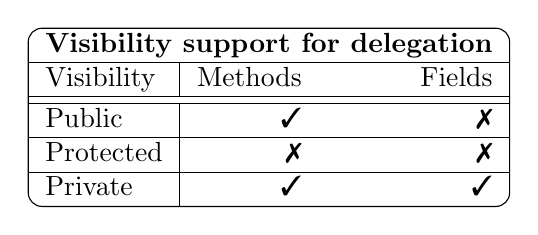
\begin{tikzpicture}
\node (table) [inner sep=0pt] {
\begin{tabular}{l|rr}
  \multicolumn{3}{c}{\cellcolor{white}\bfseries Visibility support for delegation} \\
  \hline
Visibility &  Methods & Fields   \\\hline\hline
Public     &  \ding{51} &  \ding{55} \\\hline
Protected  &  \ding{55} &  \ding{55} \\\hline
Private    &  \ding{51} &  \ding{51}
\end{tabular}
};
\draw [rounded corners=.5em] (table.north west) rectangle (table.south east);
\end{tikzpicture}
\caption{Visibility support for delegation}
\label{visibilityTable}
\end{wraptable}
Interface-delegation does not support all of Javas visibility features. Field-access cannot be delegated. Therefore public field access is only possible on the child and not on any of the parents. The biggest problem is protected access because it is inherited with class extension. Private visibility is not meant to be inherited at all so this is not a problem for delegation. See table \ref{visibilityTable} for a quick overview.



\begin{figure}[H]
\begin{lstlisting}[language=java]
class Lit {
  private Integer _x;
  public Integer getX() {
    return _x;
  }
  public Lit(Integer X) {
    _x = x;
  }
}
class LitPrint {
  private Lit _parent;
  public LitPrint(Integer x) {
    _parent = new Lit(x);
  }
  public String print() {
    return _parent.getX().toString();
  }
}
class LitCount {
  private Lit _parent;
  public LitCount(Integer x) {
    _parent = new Lit(x);
  }
  public Integer count() {
    return 1;
  }
}
class LitPrintCount {
  private LitPrint _parentPrint;
  private LitCount _parentCount;
  public LitCount(Integer x) {
    _parentPrint = new LitPrint(x);
    _parentCount = new LitCount(x);
  }
  public Integer count() {
    return _parentCount.count();
  }
  public Integer print() {
    return _parentPrint.print();
  }
}
\end{lstlisting}
\caption{Delegation implementation of the example with the type \lstinline{Lit}}
\label{delegationExample}
\end{figure}


\section{Our Solution}

\label{suggestedEPSolution}

Our Solution features: a class that contains the \emph{object algebra interface}, the result class interface (\emph{aggregation interface}) and an implementation of the \emph{object algebra}. Surrounding code uses the \emph{object algebra interface} to factorize members of this family that implement the \emph{aggregation interface}. The implementation of the factorization is the \emph{object algebra}, which can be exchanged.

Note that code-examples in this chapter are part of a valid solution to the Expression Problem developed by us. The names of the interfaces and classes are chosen to fit the aimed solution (see figure \ref{combinedClass}.

\subsection{Aggregation Interface}

We use \emph{object algebras} as a factory for classes with a collection of operations (\emph{aggregation classes}). This solution returns an aggregated interface with all operations that are needed, which is different from that proposed by Oliveira et. al. where the object algebras return a different result interface for every operation. This makes it possible for methods of the implementing classes to depend on each other and share state variables (see figure \ref{aggregationInterfaces}).

The \emph{aggregation interface} defines all of the operations that the \emph{aggregation class} has, which is the same way that it is handled in general Java context. The surrounding code addresses just the \emph{aggregation interface} and there is no modification needed.

\begin{figure}[h]
\begin{lstlisting}[language=java]
    public interface Methods {
      public String print();
    }
    public interface Methods2 extends Methods {
      public Integer count();
    }
\end{lstlisting}
\caption{Aggregation interface (\lstinline{Methods}) and an extended aggregation interface (\lstinline{Methods2})}
\label{aggregationInterfaces}
\end{figure}

\subsection{Object Algebra Interface}

\label{abstractParameter}

In order to generate objects based on the aggregation interface we need an object algebra that factorizes them. This algebra needs a factory method for every type. Types are identified by their algebraic signature \cite{Oliv-Extensibility-2012}. This means that every type has unique name and parameter types. Parameters can either be abstract or concrete. Abstract parameters differ from concrete parameters in that they refer to the most specific interface in an extension hierarchy, which means the interface of the implementing object algebra. This is similar to the \emph{ThisType} extension proposed by Foster in \emph{Rupiah} \cite{Foster-Rupiah-2001}. The abstract parameter is referenced by a dynamic type parameter "A"\footnote{"A" is a convention. This only means it is dynamic mapped by the object algebra that implements the interface}. The return class of the factory methods also has the abstract type "A" as it represents the \emph{aggregation interface} (see figure \ref{algebraInterfaces}).

\begin{figure}[h]
\begin{lstlisting}[language=java]
    public interface Types <A> {
      public A lit(Integer x);
    }
    public interface Types2 <A> extends Types <A> {
      public A add(A e1,A e2);
    }
\end{lstlisting}
\caption{Interfaces for algebras with the signature of the types}
\label{algebraInterfaces}
\end{figure}

\subsection{Object Algebra}

The main part of the object algebra is to instantiate the dependencies like super-classes of a called type and then instantiate the called type and make the dependencies available. The concrete implementations of the \emph{aggregation interface} are done using anonymous classes\footnote{Anonymous classes are desugared by the Java preprocessor into real classes with all available \emph{final} variables as private fields so they can be accessed within the anonymous class} within the object algebra methods (see figure \ref{algebraImplementation}). This technique is employed to keep users from specifying concrete classes instead of interface in their code; because referencing super-types does not work with \emph{delegation} which is used use for \emph{multiple inheritance}.

In figure \ref{algebraImplementation} in the Lit.print()-implementation we can either use \_instance2 or \_instance3 to delegate to. Coincidentally, both refer to the same operation in our example, but this can differ in another environment. To find the best ancestor for delegation one should use a linearization like that suggested by Bracha \cite{Bracha-Mixin-1990} for Mixins.

\begin{figure}[H]
\begin{lstlisting}[language=java]
public class Algebra4 implements Types <Methods2> {
  public Methods2 add(final Methods e1,
                      final Methods e2){
    final Methods _instance =new Algebra3().add(e1,e2);
    return new Methods2() {
             public Integer count() {
                 return e1.count() + 1 + e2.count();
             }
             public String print() {
                 return _instance.print();
             }
         };
  }
  public Methods lit(Integer x) { 
    final Methods2 _instance2 = new Algebra2().lit(x);
    final Methods _instance3 = new Algebra3().lit(x);
    return new Methods2() {
             public Integer count() { 
                 return _instance2.count();
             }
             public String print() { 
                 return _instance3.print();
             }
         };
  }
}
\end{lstlisting}
\caption{The resulting Algebra-class for the third extension (Algebra2 and Algebra3 likewise)}
\label{algebraImplementation}
\end{figure}

\subsection{Dynamic Dispatch}
\label{dynamicDispatch}

As Tempero et. al. point out, there are some limits to multiple inheritance with delegation \cite{Tempero-Multiple-2000}. We developed a workaround\footnote{The workaround is available online \cite{Peuscher-GitHub-EP-2014}} for the limit of \emph{dynamic dispatch} for \emph{dependent methods} (called \emph{self-calls} by Tempero et. al.). It has some downsides (see section \ref{discussionDynamicDispatch}) but works as expected.

The main idea of dynamic dispatch with delegation is to have a field of the original object in every delegation super-object. Therefore, the original-object has to be injected into all classes.

To achieve this we have to alter the aggregation interface. We add a setter with a generic type that extends from the according \lstinline{Methods} (because we do not know the last extension at this point). The visible methods of this generic type are the same as the ones from the \lstinline{Methods} interface itself (see figure \ref{dynamicDispatchMethods}).

\begin{figure}[H]
\begin{lstlisting}[language=java]
public interface Methods {
  public String print();
^\Hiline^  public <B extends Methods> void setSelfRef(B selfRef);
}
public interface Methods2 extends Methods {
  public Integer count();
^\Hiline^  public <B extends Methods2> void setSelfRef(B selfRef);
}
\end{lstlisting}
\caption{Dynamic dispatch: Adding a setter for the original object with a dynamic type \emph{B}. Needs to be done for every \lstinline{Methods} interface}
\label{dynamicDispatchMethods}
\end{figure}

With every new Methods interface a new setter has to be introduced and implemented. When called, Java calls the method with the best matching\footnote{\emph{best matching} means if an interfaces extends another interface and both could match on a method, the method with the extending class referenced is called} interface. The setter of every super interface therefore, has to be implemented even though it will not be called. The correct setter injects the original object into every super object, which inject the original object into their super objects and so on. Within the factory method the factorized object is injected into its super objects, which they then transfer into their super objects and thus overwrite the existing reference. This means that the last object to be factorized overwrites all references in every super object.

Dependent methods that call other methods of the calls only have to do their calls on the selfRef-object.

\subsection{Visibility}

Although the support for public fields, protected methods and protected fields is considered not possible (see section \ref{backgroundVisibility}), we can work out a method to support all of these three visibilities for entities.

To support public fields, all public fields of a super class have to be copied into the extending class and the access within every method to the public fields have to be done with getters and setters on the selfRef-field.
Although difficult, access to protected fields can also be made possible. Therefore, instead of setting the selfRef-object to the previous object, the selfRef would be a special instance that saves all public and protected state fields, implements all public and protected methods of the object and that is only known to the super classes and the class itself. The methods are split into two interfaces for public and protected methods\footnote{protected field access is desugared to getters and setters} and another interface that adds the \lstinline{setProtectedRef()}-methods for the delegated objects. A new anonymous class is then instantiated and injected with the setProtectedRef-methods (see figure \ref{visibilitySupportSolution}). Even dynamic dispatch with protected methods is possible with this solution.

\begin{figure}[H]
\begin{lstlisting}[language=java]
public interface PuMethods // public methods
    extends IntAlg.PuMethods {
  public Integer count(); }
public interface Methods
    extends PuMethods,IntAlg.Methods {
  public <B extends PrMethods>
    void setProtectedRef(B selfRef); }
public interface PrMethods // protected methods
    extends PuMethods,IntAlg.PrMethods {
  public String _getComment();
  public String _setComment(); }
public class Algebra implements Types<Methods> {
  public Methods lit(final Integer x) {
    public function Lit(final Integer x) {
      final IntAlg.Methods _super
        = IntAlg.Algebra().lit(x);
      final Methods _instance = new Methods {
        private PrMethods selfRef;
        public function setProtectedRef(PrMethods selfRef)
          { selfRef = selfRef;
          _super.setProtectedRef(selfRef); }
        // ... implementation of public methods
    }
    PrMethods selfRefInstance = new PrMethods() {
      private String _comment;
      public String print(String prefix) {
        return _instance.print(prefix); }
      public String _getComment() { return _comment; }
      public String _setComment(String c){ _comment = c;}
      public Integer count() {
        return _instance.count(); }
    };
    _instance.setProtectedRef(selfRefInstance);
    return _instance; }
}
\end{lstlisting}
\caption{Solution to support protected methods and fields with delegation applied to the first extensions in the example in section \ref{example}.}
\label{visibilitySupportSolution}
\end{figure}

In chapter \ref{chapterOurSolutionSyntaxExtension} we develop a SugarJ library that is supposed to generate most of the code. Because of lack of time we have not finished the SugarJ library with the support for this visibilities. There are modifications needed in the interfaces, therefore the result of this chapter would look different. In the future code examples we will ignore the solution as it would make the understanding of the SugarJ library much more difficult.

\subsection{Usage}
\label{combiningTheParts}
To just enumerate the interfaces and algebras would be very confusing. To overcome this we suggest a form that defines the interfaces and classes into a combined class (see figure \ref{combinedClass}).

To address the interface of expressions of this family, one uses \lstinline{[Familyname].Methods}. The object algebra is available with a singleton pattern. This is used not only for convenience, but also because the family class is not stateful and to minimize memory usage. A user calls the singleton and gets the algebra of type \lstinline{[Familyname].Types<[Familyname].Methods>} that he uses for initialization of the expression.

\subsubsection*{Extending Families}
\label{extendingFamilies}

To extend this family the developer creates a new outer class where the \lstinline{Methods}- and \lstinline{Types<A>}-interface\footnote{In terms of consistency the interfaces should be extended even when empty}, as well as the algebra and the singleton (that returns the algebra), are located. The \lstinline{Methods}- and \lstinline{Types<A>}-interface implement all the \lstinline{Methods}- and \lstinline{Types<A>}-interfaces of the families that are to be combined. The algebra implements the \lstinline{Types<Methods>}-interface. New types are added in the \lstinline{Types<A>}-interface (and accordingly their implementation in the algebra). The \lstinline{Methods}-interface has the setSelfRef-method (see figure \ref{dynamicDispatchMethods}) and the newly added methods. The algebra has to implement every type and in every type every method of the \lstinline{Methods}- and \lstinline{Types<A>}-interface and either implement its own methods or delegate every method call (see figure \ref{dynamicDispatchAlgebra}). All types have to be implemented, their creation is not delegated. The references have to be modified from the previous examples to meet this structure (e.g. instead of Methods2: [Familyname].Methods, instead of new Algebra2(): [Familyname].algebra(), etc.).

\begin{figure}[H]
\begin{lstlisting}[language=java]
^\HilineBackground^public class [Familyname] {
^\HilineBackground^  ^\HilineTypessmall^public interface Types<A> {
^\HilineBackground^  ^\HilineTypessmall^  [...Types...] // see figure ^\color{gray}\ref{algebraInterfaces}^
^\HilineBackground^  ^\HilineTypessmall^} 
^\HilineBackground^  ^\HilineMethodssmall^public interface Methods {
^\HilineBackground^  ^\HilineMethodssmall^  [...Methods...] // see figure ^\color{gray}\ref{dynamicDispatchMethods}^
^\HilineBackground^  ^\HilineMethodssmall^} 
^\HilineBackground^  ^\HilineAlgebrasmall^public class Algebra implements Types<Methods> { 
^\HilineBackground^  ^\HilineAlgebrasmall^  [...Type-Implementation...] // see figure ^\color{gray}\ref{dynamicDispatchAlgebra}^
^\HilineBackground^  ^\HilineAlgebrasmall^}
^\HilineBackground^  protected static Algebra _algebra;
^\HilineBackground^  public static Algebra Algebra()
^\HilineBackground^  { 
^\HilineBackground^    if(_algebra == null)
^\HilineBackground^      _algebra = new [FamilyName]().new Algebra();
^\HilineBackground^    return _algebra;
^\HilineBackground^  }
^\HilineBackground^}
\end{lstlisting}
\caption{Combining algebra interface (\emph{Types}), resulting family interface (\emph{Methods}), algebra (\emph{Algebra}) and Singleton for the algebra}
\label{combinedClass}
\end{figure}

\begin{figure}[H]
\begin{lstlisting}[language=java]
  Int.Algebra algebra = Int.Algebra();
  Int.Methods exp = 
    algebra.sub(algebra.lit(2),algebra.lit(1));
\end{lstlisting}
\caption{Usage of the solution.}
\label{combinedClassUsage}
\end{figure}

\begin{figure}[H]
\begin{lstlisting}[language=java]
public class Algebra4 implements Types2<Methods2> {
  // Lit-implementation
  public Methods lit(Integer x) {
    final Methods2 _instance2 = new Algebra2().lit(x);
    final Methods _instance3 = new Algebra3().lit(x);
    Methods2 instance = new Methods2() {
^\Hiline^      private Methods selfRef = null;
^\Hiline^      public <B extends Methods> void
^\Hiline^        setSelfRef(B selfRef) {}
^\Hiline^      public <B extends Methods2> void
^\Hiline^        setSelfRef(B selfRef) {
^\Hiline^          this.selfRef = selfRef;
^\Hiline^          _instance2.setSelfRef(selfRef);
^\Hiline^          _instance3.setSelfRef(selfRef);
^\Hiline^        }
      public Integer count() {
        return _instance2.count();}
      public String print() {
        return _instance3.print();}
    };
^\Hiline^    instance.setSelfRef(instance);
    return instance;
  }
  // Add implementation omitted
  public Methods2 add(final Methods2 e1,
                      final Methods2 e2)
    { /* ... */ }
}
\end{lstlisting}
\caption{Dynamic dispatch: \emph{Original object setter} implementation and application of the original object on super-objects. Compare to figure \ref{algebraImplementation}. Note that \emph{Add} has been omitted for clarity reasons.}
\label{dynamicDispatchAlgebra}
\end{figure}

\subsection{Solution to the Problem}

Below is a list of checks used to determine if our solution is a valid solution to the Expression Problem, as proposed by Wadler and Odersky \cite{Wadler-Expression-1998, Odersky-Expression-2005}:

\begin{itemize}
  \item \emph{Extensibility in both dimensions}: The solution can be extended by either new operations or new data variants (types). This is shown in section \ref{extendingFamilies} "Extending Families".
  \item \emph{Strong static type safety}: Static type safety is provided as there are neither explicit casts nor explicit type checks needed.
  \item \emph{No modification or duplication}: Although there is much boilerplate code that comes with every extension the code in previous packages is not being touched when extended.
  \item \emph{Separate compilation}: We do not need code to be recompiled on extension because every package refers only to its own or its super interfaces and classes.
  \item \emph{Independent extensibility}: With delegation instead of inheritance the extensions can be combined independently without touching existing code.
\end{itemize}

Our solution complies with all of the requirements above. Therefore, it considered it a valid solution.

\section{Related work}

There are plenty of solutions to the Expression Problem in literature. These can be divided into two groups: solutions that rely on syntax extensions and solutions that do not rely on syntax extensions. In this section we compare our work on the Expression Problem with solutions that do not rely on syntax extensions.

\subsection*{The Expression Problem Revisited}

\emph{The Expression Problem Revisited} is a paper about a solution to the EP by Torgersen published in 2004 \cite{Torgersen-Expression-2004}.
Torgersen's definition of a valid solution is less restrictive. It allows for code to be recompiled but not changed and allows casting under the condition that every combination has to be handled. The restrictions proposed by Wadler \cite{Wadler-Expression-1998} do not allow solutions to depend on recompilation and they force solutions to use static type safety. So, although the restrictions for recompiling code are looser, everyone of Torgersen's solutions meet the strict requirements of Wadler for recompiling code and therefore, we consider the requirements met. We only compare the first solution because it has a very similar structure to ours. The comparison to the other three solutions has been presented by Torgersen in his paper.

Torgersen's first approach is (as is ours) \emph{data-centered}, which means the structure, from where the extensions are derived, are types. It uses type parameters to make sure that the constructors are called with the correct (sub-)type. Extension of classes is similar to generic sub-typing except in the case of the type parameter, which has to be transferred. To eliminate F-Bounds another sub-type without type parameters is needed. This is done by using an abstract factory to generate types of the correct family.

The difference between Torgersen's and our approach is mostly the inheritance. Our approach features independent extension, which we made possible by using delegation. The result is that we do not need type parameters in our \lstinline{Methods}-interface. Also we do not need the F-Bounds free subtype as our types are already F-Bound free. Instantiation with abstract factories (object algebras) is generally handled in the same way.
Unfortunately delegation for inheritance does not support \emph{dynamic binding}. We overcame the \emph{dynamic binding} problem but it comes with some downsides which are explained in section \ref{discussionDynamicDispatch} whereas the solution by Torgersen uses Java inheritance which does not have these problems.

\subsection*{Some Challenging Typing Issues in Object-Oriented Languages: Extended Abstract}

{Some Challenging Typing Issues in Object-Oriented Languages: Extended Abstract} is a paper about an extended Java language that solves the EP among other things by Bruce published in 2003\cite{Bruce-Typing-2003}.
Bruce's solution depends on a Java language extension named "Rupiah"\cite{Foster-Rupiah-2001}. The extension supports a concept called \emph{ThisType}, which adds a dynamic type to every class. This type is comparable to the dynamic field "this" and describes the type of an instantiated object. With \emph{ThisType}, a super-class is able to reference the type of a derived sub-class, which solves the problem of \emph{abstract types} that object algebras were used to solve. Unfortunately Java does not yet include a feature similar to ThisType.

\section{Discussion}

This chapter discusses the usage of delegation in lieu of regular inheritance. It discusses a view on the advantages and the disadvantages that come with multiple inheritance and delegation.

\subsection{Delegation}
We used delegation to support the requirement of \emph{independent extensibility} \cite{Odersky-Expression-2005, Oliv-Extensibility-2012}. The solution of Oliveira et. al. supports some kind of independent extensibility, but there were some difficulties in its implementation. Also it is not very easily generated because the needed background-knowledge of the implementation needs to be used in the generation process. Also the use of this solution is very inconvenient for the surrounding code. Another point that kept us from using a solution like the one from Oliveira et. al. is that it does not fully support depending methods. We worked out a solution how they could work and found it to be even more difficult to generate than the independent extensibility.

Delegation comes with some overhead in memory usage, instantiation speed and usage speed. This is because for every inheritance there has to be at least another object that is to be kept in memory. This can be a problem in very complex inheritance trees. Also, because operations are delegated through the inheritance tree, the execution of them is slightly slower.

On the other hand, delegation gives us the possibility to extend types independently and support multiple inheritance. Also, with our solution to dynamic dispatch for delegation, many of the problems delegation brings, are erased.

\subsection{Dynamic Dispatch}
\label{discussionDynamicDispatch}

When not used properly \emph{delegation} does not work exactly like inheritance. We tried to adapt the \emph{dynamic dispatch} of inheritance to delegation. It works as one would expect inheritance to work. Therefore intern method calls have to be done on an extra fields instead of the current namespace or with the \lstinline{this}-reference. With this workaround we are able to use \emph{multiple inheritance}-like extension in Java.

Our solution to dynamic dispatch for delegation has some downsides that one should keep in mind when using it.
\begin{itemize}
  \item \emph{Code}: Dynamic Dispatch increases the boilerplate code very much. This depends on the structure and entities. In our example the whole code was increased by about 45\%, but as we want to generate the code anyway this is not that much of a problem.
  \item \emph{Convenience}: The access to the dependent methods have to be executed on a instance field instead of implicitly by calling the namespace-method. Also, when providing self-reference (e.g. when implementing Observer pattern\cite{Gof-Design-1993}) it has to be done with the same field. This might be overcome with desugaring.
  \item \emph{Performance}: In complex extension combinations the instantiation could take more time and more memory. However, as the solution just copies references we believe that this not have too much of an impact on both memory time and speed.
  \item \emph{Visibility}: Our main idea to overcome the missing \emph{dynamic dispatch} is to set the main object into every super class. We cannot use visibility to limit the external access because the algebra would not have access to set it in the first place.
\end{itemize}

Excessive \emph{boilerplate code} and poor \emph{convenience} are two of the most important problems. Our solution sets out to solve these. In the next chapter we present a solution that addresses both of these difficulties by implementing a SugarJ library that generates most of the boilerplate code and modifies the written code so that a user does not have to worry about the special solution.






%%%%%%%%%%%%%%%%%%%%%%%% Syntax Extension





\chapter{Syntax Extension For The Solution}

\label{chapterOurSolutionSyntaxExtension}

In this chapter we describe the development of a SugarJ library that features a syntax extension for the solution to the \emph{Expression Problem} that we described in the previous chapter. With this work we provide an experience report on working with SugarJ to develop libraries that provide domain specific languages \cite{Erdweg-SugarJ-2011}. The solution should meet the requirements, that users generally have on languages. In our solution we compare the syntax with different applicable \emph{Cognitive Dimensions} to ensure these requirements are met \cite{Green-Cognitive-1996}.

The solution to the Expression Problem, described in the previous chapter, is a great fit to develop a syntax for, because it was developed specifically to generate most parts of the code. We are developing a syntax that represents the roles of the solution and we are then developing a Stratego ruleset that provides the rewriting for the solution. All the work is done in the SugarJ environment, which makes it easy to use the solution in an IDE.

SugarJ is a very young framework and most of the work in literature to-date, which is written by the authors of SugarJ, is about extending, describing possible use cases and working on the framework \cite{Fehrenbach-Retrofitting-2011, Erdweg-Composition-2012, Erdweg-Editor-2011, Erdweg-SugarHaskell-2012, Erdweg-Questionnaire-2013}. With this in mind, we set out to describe, in this section, what’s involved from a new users perspective of SugarJ - from learning the concepts through to implementing a working library of a special use case.

\section{Background}

To develop this syntax extension we use SugarJ, which is a framework used to extend syntax in Java. SugarJ itself relies on \emph{Syntax Defintion Formalism} and \emph{Stratego/Xt}. To describe the types we use \emph{algebraic signatures}. We compare our syntax in \emph{Cognitive Dimensions} to ensure the relevant metrics are met.

This section introduces the used technologies.

\subsection{SugarJ}

SugarJ is a framework which allows seamless integration of syntactic sugar (for Java) into an IDE such as Eclipse \cite{Erdweg-SugarJ-2011}. It uses the \emph{Spoofax framework}, which makes new syntax definitions just in time available in the editor. SugarJ uses syntax definition formalism (SDF) to provide new non-terminals and keywords for language detection \cite{Heering-SDF-1989}. It then uses Stratego/XT rules and strategies to manipulate the generated ATerm tree and afterwards export the valid code in Java \cite{Kats-Spoofax-2010, Brand-ATerms-2000}.

SugarJ uses SDF to define syntax (see example in figure \ref{exampleSDFJavaClassDecHead}). There is already a SDF of Java language available in the SugarJ repository where one can lookup design and structure of the language and find information about how to derive ones own language extensions \cite{Heering-SDF-1989, Brand-SDF-2007, Java-SDF-2014}. With this definition, an IDE that supports the Spoofax framework is able to parse, verify and syntax highlight code that is written in this new syntax.

\begin{figure}[H]
\begin{lstlisting}[language=java,breaklines=false]
( Anno | ClassMod )* "class" Id TypeParams? Super? 
    Interfaces? -> ClassDecHead {cons("ClassDecHead")}}.
\end{lstlisting}
\caption{Example of the Java class head with \emph{SDF} \cite{Java-SDF-2014}}
\label{exampleSDFJavaClassDecHead}
\end{figure}

In the second step, SugarJ uses Stratego/XT to rewrite parts of the ATerm (tree representation of a whole syntax representation in SDF) of a language with various rules to remove every non-terminal that might be added by the previous SDF \cite{Stratego-Manual, Kats-Spoofax-2010, Brand-ATerms-2000, Visser-Stratego-2003}.

\begin{figure}[H]
\begin{lstlisting}[language=java,breaklines=false,morekeywords={field1,field2,field3,annot,typeParams,result,methodName,params,throws,body,rest},keywordstyle=\bfseries\color{OliveGreen}]
function-search-methods-bodyparts: [] -> []
function-search-methods-bodyparts:
  [FieldDec(field1,field2,field3) | rest]
    -> <function-search-methods-bodyparts> rest
function-search-methods-bodyparts:
  [MethodDec(MethodDecHead(annot,typeParams,result,
      Id(methodName),params,throws),body) | rest]
    -> <concat>[[
		   AbstractMethodDec(annot,typeParams,result,
		     Id(methodName),params,throws)
		          ],
		          <function-search-methods-bodyparts> rest]
\end{lstlisting}
\caption{Example of a \emph{Stratego/XT} rule that searches and replaces methods by according abstract methods and removes fields to generate the contents of an interface from a class}
\label{exampleStrategoClassInterfaceTranslation}
\end{figure}


SugarJ uses these two technologies, in combination with the Spoofax framework, to define new domain languages (SDF), that an IDE can use to utilize (Spoofax), and afterwards transform into valid Java code\footnote{There are also frameworks like SugarJ for \emph{Haskell} (SugarHaskell) and \emph{Prolog} (SugarProlog)} (Stratego). This process is called \emph{Desugaring}, because syntactic sugar, matched with a language extension via SDF is transformed from generic code into another language that assigns the idea of the domain language to it.


\subsection{Algebraic Signature}

\label{albegraicSignature}

An \emph{algebraic signature} is the structure of a type and contains its return type, its parameters and its name {Oliv-Extensibility-2012}. Parameters can either be abstract of concrete. Abstract parameters represent the current interface that factorizes the main object. In the example described in section \ref{example}, the signature of "Lit" is \lstinline{Lit: Integer -> Methods} and the signature of "Add" is \lstinline{Add: Methods x Methods -> Methods}. The algebraic signature of a type is the same among family inheritances, although the \lstinline{Methods}-type is abstract so that it is adapted to the interface of the according family.

\subsection{Cognitive Dimensions}
\label{backgroundCognitiveDimensions}

To get a neat integration and a wide usage of a language extension one needs to check the integration features with the existing language.

This is done using \emph{cognitive dimensions}, which describe a set of features and rules that are used to check the performance of the a language against standard metrics \cite{Green-Cognitive-1996}. \emph{Cognitive dimensions} are also used when designing new syntax to ensure the new code will meet the quality of the code.

\subsubsection*{The \emph{Consistency} Metric}

The consistency of a language can be determined by how easy it is to adapt all features of a language while being familiar with only some features of the language. It is very important that consistency is considered when implementing syntax extensions that extend a complete language with syntactic sugar. After all, the main goal of syntax extensions is to simplify features that would otherwise be difficult to implement.


\subsubsection*{The \emph{Viscosity} Metric}

The viscosity of a language describes the effort that is required to perform a single change. As long as lowering the effort does not conflict with the readability of the code, then the lower the effort - the better this condition is met.


\subsubsection*{The \emph{Progressive Evaluation} Metric}

Progressive evaluation describes if a developer gets feedback from a partially-complete program.


\section{SugarJ Library}

In this chapter we define a new syntax that is stripped down to the essential parameters that are needed for a solution of the Expression Problem. Afterwards we develop a SugarJ library which transforms the new syntax to our solution of the Expression Problem in chapter \ref{theProblem}.

Note that code-examples in this chapter use the new syntax extension.

\subsection{Family Syntax}

A \emph{Family} represents an expression or an extension to an existing expression (distinguished by wether the family has an "extend"-clause or not). It is a structure that couples the entities to enable them to be part of the expression. Expression elements have the same interface. In each family, every class implements the family interface. Every public operation that exists in one of the elements of the family has to be in every other family. Families can extend each other independently. Every derived family inherits the public methods of the super families and the elements have to implement the missing methods. Methods in families can be overwritten.

A family of the third extension of our example in section \ref{example}, (where IntSub and IntCount are the first and second extending families) will only implement the missing method \lstinline{count()} on the entity \lstinline{Add} (See figure \ref{thirdExtensionFamily}). The classes and methods that are not implemented are delegated to their extended family instances. The family \lstinline{IntAddCount} in figure \ref{thirdExtensionFamily} includes every type of the extended families \lstinline{IntAdd} and \lstinline{IntCount}. If these families are implemented like the example in section \ref{example}, \lstinline{IntAdd} would have the types \lstinline{Lit} and \lstinline{Add} and the operation \lstinline{print()}, whereas \lstinline{IntCount} would have the type \lstinline{Lit} and the operations \lstinline{print()} and \lstinline{count()}. The new family \lstinline{IntAddCount} would then have the types \lstinline{Lit} and \lstinline{Add} and the operations \lstinline{print()} and \lstinline{count()}. When more than one extension implement the same operation for the same type, the call for this method is delegated to the \emph{last} extension in the list of extending families.

\label{familyDependentType}
To reference to an \emph{abstract parameter} (see section \ref{abstractParameter}) we use the family name as type. This does not change the \emph{algebraic signature} (see section \ref{albegraicSignature}) of a given type since the definition of algebraic signature says that \emph{abstract parameters} do not change among inheritance.

Parameters of the algebraic signature are available in the scope of every method in its family class. They are desugared to final private fields in the class, so they can be used just like any other final field (see figure \ref{thirdExtensionFamily}).

\begin{figure}[h]
\begin{lstlisting}[language=exprExt]
family IntAddCount extends IntAdd,IntCount {
  family class Add (IntAddCount e1,IntAddCount e2) {
    public Integer count () {
      return new Integer(e1.count() + 1 + e2.count());
    }
  }
}
\end{lstlisting}
\caption{The third extension of the example (see section \ref{example}) with families. \lstinline{e1} and \lstinline{e2} are available as final fields in the methods of the family class.}
\label{thirdExtensionFamily}
\end{figure}


\subsection{Defining the Syntax Extension}
We define the syntax extension in SDF. The SDF-matching generates an ATerm that represents the whole structure of the code. It uses constructors that have the parameters of the variable parts in the entity. The other structure type is "list". Based on the definition showed in figure \ref{exampleSDFJavaClassDecHead} - a constructor of \lstinline{ClassDecHead} would for example be \lstinline[breaklines=false,morekeywords={field1,field2,field3,annot,typeParams,result,methodName,params,throws,body,rest},keywordstyle=\bfseries\color{OliveGreen}]{ClassDecHead([Public()],"Lit",None(),None(),None())}. A list will be indicated by brackets seen in this example at the visilibity: "[Public()]".

An entry point for the existing non-terminals (constructors are non-terminals) in the Java language is required. For this we choose the \emph{JavaTypeDec} as it is the top level\footnote{On top of that are only imports and namespaces which cannot be matched by SugarJ, because they are used to define which SugarJ-library will be used.} of declaration in Java, where among some others every class and interface is declared. We define a new keyword "family" and bring it into context with our own structure. To avoid reinventing the wheel, we referred to the generic Java non-terminals as often as possible (e.g. JavaClassBody, we do not have to redefine what a class-body contains). After that, the new syntax can be matched. Figure \ref{sdfFamilies} shows the whole SDF for our syntax extension.

To define the syntax, we first have to define the keywords. In our case we only have to define the "family". The lexical restrictions define which characters can be (or cannot be) next to the keyword to let it still count as keyword. Afterwards we can use the keyword in the syntax declaration. The structure of the family syntax declaration orientates on the syntax declaration of Java classes. The entry point can be seen in line 7: JavaTypeDec is the top level declaration type. This means that families are expected on the top level of a file, right beneath the imports, where one would generally write class and interface declarations. The exit point is in line 21 and 22 where the JavaClassBody is referenced. This means that a generic JavaClassBody-element (like fields and methods) can be placed inside a \emph{family class}.

\begin{figure}[H]
\begin{lstlisting}[language=java,breaklines=false]
  lexical syntax
    "family" -> JavaKeyword
  lexical restrictions
  	  "family" -/- [A-Za-z0-9\_\$] 
  sorts FamilyDecHead FamilyBody FamilySuper FamilyDec
  context-free syntax
    FamilyDec -> JavaTypeDec
    "family" FamilyClassId FamilySuper? ->
      FamilyDecHead {cons("FamilyDecHead")}
    JavaID -> FamilyClassId {cons("FamilyClassId")}
    JavaID -> 
      FamilyFamilyClassId {cons("FamilyFamilyClassId")}
    FamilyDecHead FamilyBody ->
      FamilyDec {cons("FamilyDec")}
    "{" FamilyBodyDec* "}" ->
      FamilyBody {cons("FamilyBody")}
    "extends" { FamilyClassId ","}+ ->
      FamilySuper {cons("FamilySuper")}
    FamilyClassDec ->
      FamilyBodyDec {cons("FamilyBodyDec")}
    FamilyClassDecHead JavaClassBody ->
      FamilyClassDec {cons("FamilyClassDec")}
    "family" "class" FamilyFamilyClassId
        "(" {FamilyClassFormalParam ","}* ")" ->
      FamilyClassDecHead {cons("FamilyClassDecHead")}
    JavaID JavaVarDecId ->
      FamilyClassFormalParam {cons("FamilyClassFormalParam")}
\end{lstlisting}
\caption{Actual implementation of the matching SDF for the syntax extension for "families". This is an example in SDF-code.}
\label{sdfFamilies}
\end{figure}


\subsection{Rewriting the Syntax Extension to Java-Code}
The rewriting rules have to be defined strict\footnote{On the top level one can generate either a list or a top level element, which is important if you want to generate more than just one top level element. However, we found this as the only exception.}. Unnecessary Brackets are not automatically ignored. We found the use of the embedded syntax for Java code to be too restrictive and we needed to generate new structures based on derived code, so we chose to use only ATerm matching and rewriting. The Stratego manual \cite{Stratego-Manual} is very helpful, especially for the documentation of built-in strategies.

For an example of a \emph{Stratego} rule, see figure \ref{exampleStrategoClassInterfaceTranslation}. The code of our \emph{Stratego} rules are about 1200 lines. The entry point of the rewriting is the \lstinline{desugar-family} strategy, which generates the outer Java class of our solution.

\begin{figure}[H]
\begin{lstlisting}[language=java,breaklines=false,morekeywords={familyname,super,familyClasses},keywordstyle=\bfseries\color{OliveGreen}]
  desugar-family:
    FamilyDec(
      FamilyDecHead(FamilyClassId(familyname), super)
    , FamilyBody(familyClasses)
    ) ->
      <concat> [[
        ClassDec(
          ClassDecHead([Public()], Id(familyname)
          , None(), None(), None())
        , ClassBody([
            <desugar-family-type-interface> (
              familyname,super,familyClasses)
          , <desugar-family-function-interface> (
              familyname,super,familyClasses)
          , <desugar-family-class> (
              familyname,super,familyClasses)
          , FieldDec(
              [Protected(), Static()]
            , ClassOrInterfaceType(
                TypeName(Id("Algebra")), None())
            , [VarDec(Id("_algebra"))])
          , <desugar-family-algebra> (familyname)
          ])
	     )]
      , <desugar-family-sugar>
          (familyname
            , <family-super-list>super,familyClasses)
      ]
\end{lstlisting}
\caption{First rule that is applied and desugars a \emph{family} declaration. It generates the outer class and delegates the implementation of the different parts (interfaces and classes) to other rules. The last rule (desugar-family-sugar) generates a new SugarJ library with variable parts.}
\label{exampleStrategoClassInterfaceTranslation}
\end{figure}

We cannot cover all of the rules in this thesis. However, we will have a detailed look at the main rule (\emph{desugar-family} - see figure \ref{exampleStrategoClassInterfaceTranslation}). Within it we give a closer look about some special cases. The first part before the arrow (-\textgreater) is the matching of the ATerm. There are three variables in which the sub-terms are saved: \bfseries familyname\mdseries, \bfseries super \mdseries and \bfseries familyClasses \mdseries. \bfseries familyname \mdseries is a string with the name of the family; \bfseries super \mdseries is an ATerm that is either \lstinline{None()} or \lstinline{FamilySuper(...)}; and \bfseries familyClasses \mdseries is either \lstinline{[ ]} (empty list) or \lstinline{[FamilyClassDec(...),...]} . In the second part the \lstinline{<...>}-calls are explicit calls to rules with the next ATerm as parameter.

\subsubsection{\textless desugar-family-function-interface\textgreater, \textless desugar-family-type-interface\textgreater, \textless desugar-family-algebra\textgreater{} and FieldDec(...)}

The right side of the arrow has a very similar structure to the example in figure \ref{combinedClass}. The lines 7-24 of the example are actually used to generate the code in this example. The \lstinline{<desugar-family-type-interface>}-rule generates the object algebra interface (\lstinline{Types<A>} see \ref{algebraInterfaces}) and the \lstinline{<desugar-family-function-interface>}-rule generates the aggregation interface (\lstinline{Methods} see \ref{dynamicDispatchMethods}). Both are very simple because they just generate a fix structure with the according \lstinline{extends}-clauses as the family itself. Only the types and methods in the actual family have to be written, since the rest is inherited. "Overwriting" inherited methods does not make any difference. The \lstinline{<desugar-family-algebra>}-rule has even more static content than the two before. It generates the \lstinline{Algebra()}-singleton where only the familyname is needed. The \lstinline{FieldDec(...)}-part is part of the singleton and is the field where the single instance is saved. It is extra in this structure because when we return a list in the \lstinline{<desugar-family-algebra>}-rule, the Java pretty printer will fail with an error. It will try to parse a list in the ClassBody list that it does not expect because a list is not a ClassBodyDec.

The more difficult parts are in the \lstinline{\textless desugar-family-sugar\textgreater}-rule and the \lstinline{\textless desugar-family-class\textgreater}-rule, which is described below.

\subsubsection{\textless{}desugar-family-sugar\textgreater}
The \lstinline{<desugar-family-sugar>}-rule is used to export meta data on a special family. The proposed method is to use content from other desugarings and to define a SugarJ library within the desugaring process. The SugarJ parser will generate a SugarJ library that any other SugarJ library can include and use the rules from. The importing does not even have to be inside the SugarJ code, but rather in a (sugared) domain language file that includes both SugarJ libraries. We use this technique to export the types, methods and all super families so that an extending family knows which types and methods it has to delegate and knows to which super family it has to extend to. The SugarJ/Stratego file that the example in figure \ref{thirdExtensionFamily} generates has the following 5 rules in it:
\begin{itemize}
    \item \lstinline{typeList ("IntAlgSubCount")}: this rule returns a list of pairs of algebraic signatures of \emph{types} in this structure: (typeName,[parameterName1,parameterName2,...]).
    \item \lstinline{methodList ("IntAlgSubCount")}: this rule returns a list of pairs of \emph{methods} and their parameters in this structure: (methodName,[parameterName1,parameterName2,...]).
    \item \lstinline{typeHead (typeName,[parameterName1,...])}: Returns the type method head for the algebra and the parameters that are needed to delegate the type if it is not overwritten by the extending family.
    \item \lstinline{methodHead (methodName,[parameterName1,...])}: Returns the method head and the parameters that are needed to delegate the method if it is not overwritten by any type of the extending family.
    \item \lstinline{superList ("IntAlgSubCount")}: Returns a list of all super families that this family inherits from. This is needed for all the \lstinline{setSelfRef(...)} methods that have to be implemented (see section \ref{dynamicDispatch}).
\end{itemize}
Because the methodHead-rule and typeHead-rule return complex structures and the effort to generate the rule that would return the structures with constructors and lists would be too big, we serialize the structure into a string and on calling the rule, deserialize it. The rules for this (de-)serialization are built into Stratego and are called "write-to-string" (for serialization) and "read-from-string" (for deserialization).

The SugarJ-libraries are (fortunately) included implicitly because the families that an extension extends have to be imported explicitly. This includes the generated SugarJ libraries.

\subsubsection{\textless{}desugar-family-class\textgreater}
The \lstinline{<desugar-family-class>}-rule generates the algebra. This includes the delegation which would not work if we did not have the exported metadata from the super families. With this data the generation of types and methods is mostly simple iterating over lists and generating the delegation code where either whole types or methods of types are not overwritten. The setSelfRef-Methods that are derived by every super family are generated with the metadata that was exported by the super families.

We do not want the user to have to worry about the selfRef-implementation so we need to desugar every implicit method-call without an object and every \lstinline{this}-method-call to be redirected to the selfRef-object. For this operation we need a \emph{strategy}\footnote{A strategy is a rule, that defines how a given rule is applied.} that does not need to be applied to a fixed structure but rather a strategy that searches an ATerm for a structure and replaces the structure everywhere. There are some strategies built into Stratego that support this feature. We chose the "innermost" strategy. The call of a rule with this strategy looks like this: \lstinline{<innermost(method-code-replacements)> ATerm}. The according rule to replace every occurrence of an implicit method-call by a call on the selfRef-object is shown in figure \ref{replaceMethodBySelfRef}.

\begin{figure}[H]
\begin{lstlisting}[language=java,breaklines=false,morekeywords={familyname,super,familyClasses},keywordstyle=\bfseries\color{OliveGreen}]
method-code-replacements:
  (MethodName(Id(methodName))) ->
    Method(MethodName(AmbName(Id("selfRef"))
      ,Id(methodName)))
\end{lstlisting}
\caption{Stratego-rule to replace every occurrence of an implicit method-call by a call on the selfRef-object.}
\label{replaceMethodBySelfRef}
\end{figure}

\section{Related Work}

SugarJ is in an early stage of popularity. Therefore there are not many papers that \emph{use} SugarJ but many \emph{about} SugarJ. This section compares our work with SugarJ with the paper we found that was comparable.

\subsection{Embedding a Questionnaire DSL with SugarJ}

The paper is from Erdweg, the main founder of SugarJ, so the knowledge of him about the technology is very high \cite{Erdweg-Questionnaire-2013}. Compared to our situation, where the study of the technology can be seen as part of the work, the code is obvious superior. The semantic structuring among different files is consistent where in our work, everything is in one combined file. He uses features that we either did not know existed or did not understand their use like annotations and editor commands. On the other hand we consciously decided to not use embedded Java syntax. Our rules do not contain much static content. Therefore we decided to used plain aterm rules.

It is not surprising that the work is a sovereign example how work with SugarJ can look. Questionnaire is very great example how powerful SugarJ is.


\section{Discussion}

This section compares our syntax extension to the \emph{Cognitive Dimensions} from section \ref{backgroundCognitiveDimensions} and points the missing features with a potential solutions in the future.

\subsection{Cognitive Dimensions}

In this section we describe how well our syntax extension complies with the cognitive dimension metrics.

\subsubsection*{The \emph{Consistency} Metric}

The \emph{family syntax} meets this requirement, because it consists of classes that have mostly the same syntax and features as every other class a user would write. The context of an interface family has the same symbols as an interface would have. The binding of the classes in the family to the interface name communicates the outer interface to be met by the inner classes.

Because multiple inheritance is not part of Java, a given algorithm to delegate derived calls to the super objects is not forced. The reversed extend-order does not violate this rule, so the \emph{consistency} metric for our extension is good.

\subsubsection*{The \emph{Viscosity} Metric}

In the \emph{family} syntax, the effort for a change is very low. Because every method that is added to a class will extend the interface and every type that is defined in the family will implement the interface, it does not have to be updated explicitly. To extend a class, one simply has to define it and does not need to know if: a) it was already derived from a previous family or b) which methods have to be derived. With this feature, the viscosity metric is good.

\subsubsection*{The \emph{Progressive Evaluation} Metric}

Our draft does not support this requirement yet, because of the need for static type checks. But it would be possible in a future implementation to allow methods that have not been implemented in a type to throw an exception. Now the compiler would fail on a missing method. The metric in this case is not very good, but could be in a future revision.


\subsection{Limitations}
\label{syntaxExtensionLimitations}

There are a few limitations that our SugarJ library does not support. To some of the limitations we will provide a potential solution, to a few we only had an idea. We try to provide an estimate if it these features will be supported in the future.

\subsubsection*{Visibility}

We proposed a solution to the limits in visibility in section \ref{visibilitySupportSolution}. Because of lack of time we did not finish the implementation in SugarJ to support the visibility. This might be done in a future version of the SugarJ library.

\subsubsection*{Multiple Inheritance Linearization}

The inheritance order follows a simple reversed hierarchical order. Calls to derived methods are delegated to the first Family Interface that has the method in reversed order of the "extends" keyword. Although a linearization like with \emph{Mixins} suggested by Bracha \cite{Bracha-Mixin-1990} would have been more straight-forwarded, the implementation of this algorithm was not possible because of lack of time. The \lstinline{super}-object is also not supported and desugaring makes no sense until the multiple inheritance linearization algorithm is implemented.

For implementation of this feature in future versions of the SugarJ library the exported metadata from a family has to include the types and methods combinations, that each family implements without delegation. An algorithm implemented in the \lstinline{<find-super-method>}-rule could then decide to which super-object the delegation has to be done.

\subsubsection*{Inheritance within family members}

Subtyping of family members from other family members or from outside the family is not supported.

Delegation to super-families could also be applied to types other than the type with the same name. One could also implement multiple inheritance with this kind of specialization. The linearization of inherited methods with the same method-head would become a little bit more complex with this solution.

\subsubsection*{Instantiation and addressing of Members from the Inner Code}

Although one can instantiate new members of the same family with using the \_algebra field, the dependencies of a derived family are not met because there is no method to get to the caller family \_algebra-field.
Addressing a specific family type is also not possible.

For instantiation constructors of algebras could be equipped with the last algebra as an abstract factory. The code that creates new instances would then be desugared to use the abstract factory instead. We are not sure if this works without breaking the solution to the EP (i.e. the features that a solution has to support).

The translation from the abstract type to the concrete implementation does only work when the type matches exactly the family name. It does not work as a type parameter.

\subsubsection*{Different Qualified Type Names}

Java supports the use of different qualified type names with the use of the "import"-command. Our syntax extension only works when resulting types are addressed the same in every derived family. This is the case for family types and methods.

We believe this could be possible, but the effort would be huge because a type-checker like in the Java-compiler would be needed to resolve the imports. SugarJ has to be adapted to make it possible to match on imports. A more simple problem that could be used with a little downside would be to limit the usage to explicit \emph{class} imports.

\subsubsection*{Constructors}

Classical Java constructors are not supported. With algebraic signatures (see section \ref{albegraicSignature}) we eliminated the need for most uses of constructors in Java which is to save instantiation-variables in class-fields.

A constructor behaves a little different than other methods. One could find out the differences and emulate then in a defined constructor-method. Then when instantiating the object in the algebra, the constructor could be called with the emulated behavior.

%%%%%%%%% Experience with SugarJ

\chapter{Experience With SugarJ}
\label{sugarJChapter}

This chapter provides the experience we made with SugarJ during the development-process. It is meant to help users to decide wether or not they should use SugarJ and where possible provide workarounds to common problems we experienced.

\section{Installation and IDE}
The installation is quite straight-forwarded and through the eclipse software installation dialog very easy. The instructions can be found on the official site of SugarJ \cite{SugarJ-Homepage}. The interpreter has to be aligned in the target project, but that is all, that is needed to do by hand. When opening a .sugj-file one has a few options to start: Import an existing "Sugar", define ones own "Sugar" or use syntax that goes through the process as described (SDF matching, Stratego rewriting). The transform menu is an easy way to generate ATerms from existing code to get a feeling for ATerm-transformation of existing code in Java as well as existing SugarJ-code.

\section{Difficulties with SugarJ}
During the development the behavior of SugarJ was not always as we expected it to be. In some cases it took time to figure out how to work around the problems and in one case we just had to accept the time it costed.
\begin{itemize}
\item \emph{Equal Matching} - SugarJ adds analysis hashes as annotations to every ATerm element. This makes two similar options act not like expected and described in the Stratego-Manual\cite{Stratego-Manual}:
\begin{enumerate}
 \item The matching of a term that contains the same variable more than once to match equality between these variables will not match. The reasons are the different hash values that are attached to the elements before the rules are applied and that unify every element in the ATerm. There are two workarounds to overcome this: either match  two different variables and add a "where"-clause after the rule to compare them (see the next point) or execute the built in strategy \lstinline{<strip-annos>} to the term before the matching.
 \item The \lstinline{<eq>}-strategy that matches if two elements are the same does also not work with the ATerm because of the hash annotations.  So instead of the \lstinline{<eq>}-strategy, one should use the \lstinline{<structurally-equal>}-strategy (also built-in) that matches without comparing the annotated hash values.
\end{enumerate}
\item \emph{Debugging} - SugarJ has a console where it prints out when a desugaring goes wrong. There are two different ways that can happen in the stratego-part of the desugaring:
\begin{enumerate}
 \item The result to the transformed ATerm cannot be pretty printed. This type of error message give a hint where to look for the problem, because the term that was tried to be printed out is echoed to the console and can be analyzed. To find malicious part of the ATerm, one has compare the echoed term to the Java SDF \cite{Java-SDF-2014}. The full ATerm is echoed, therefore one has to look where the last change was. Executing \lstinline{<strip-annos>} before looking into it makes it easier to read the ATerm.
 \item The term could not be matched. The console only prints the whole ATerm that could not be matched, but no more debug-information. With the \lstinline{<write-to-string>}-strategy one is able print the ATerm into a valid output like a string in Java to see how a not matching term looks.
\end{enumerate}
\item \emph{Derive new Libraries} - In some cases it is important to extract information from a syntax extension. The syntax extension desugars a new "Sugar"-structure that can be used in future desugaring. The most simple way to translate ATerms into the new libraries is with the serialization of read-from-string and write-to-string.

As the imports of the original code inherits automatically \footnote{In Chapter 6.5 of Erdweg et. al.'s introduction of SugarJ, they wrote about the different scoping rules of imports \cite{Erdweg-SugarJ-2011}}, explicit imports of the new Sugar-library are not necessary. Erdweg et. al. announced that they might rethink this and probably change the way it works.
\item \emph{Stability of the Environment} - SugarJ is a research project. As such it is not entirely checked for its stability against every configuration. We had experienced some minor bugs that could be overcome (e.g. by deactivating "build automatically" in Eclipse) and one major bug that hindered our development about half of the time. The IDE froze randomly when text was marked. Unsaved states could not be recovered. We had to kill and restart the IDE whenever this happened. It seems like it happens only in a specific environment since it occurred after a switch of the development system and the answer to the reported bug was that it could not be reconstructed.
\end{itemize}

\section{Estimation on the Usage}

The possibility to define a new language extension in the same IDE as using it is very convenient. When it works the way it is expected the definition of domain specific language makes it easy to generate code instead of writing it. With enough experience, development processes can be automated to a huge amount and with little effort to develop.

A clear structure of the SugarJ rules is essential. There is no prescribed structure so the structure should be decided as soon as one can differentiate between parts of the development.

In the development of this thesis the stability of the environment was the most frustrating. The advantage of defining the syntax and the desugaring in the IDE where it is used gets lost if the IDE crashes too often. This seems to be environment depending as it does not happen with a different computer. The version we used was last modified in November 2013 and this version still has the stability problem.



\chapter{Use Case}

The following real life example is a proof, that in a working environment the presented solution saves much manual writing and decouples functional extensions and type extensions. All of the outlined features are included in this example.

\begin{figure}[h]
\begin{lstlisting}[language=bash,numbers=none]
ShapeSCTCircumLength.sugj           (Lines:  22)
ShapeSCTECTSACRatio.sugj            (Lines:  35)
ShapeSCTECircumLength.sugj          (Lines:  16)
ShapeSCTEllipse.sugj                (Lines:  13)
ShapeSCTTupleShapeCircumLength.sugj (Lines:  25)
ShapeSCircleTriangle.sugj           (Lines:  20)
ShapeSquare.sugj                    (Lines:  10)
-------------------------------------------------------
Total                               (Lines: 141)
\end{lstlisting}
\caption{Ensugared Code}
\end{figure}

\begin{figure}[h]
\begin{lstlisting}[language=bash,numbers=none]
ShapeSCTCircumLength.java           (Lines: 123)
ShapeSCTECTSACRatio.java            (Lines: 249)
ShapeSCTECircumLength.java          (Lines: 132)
ShapeSCTEllipse.java                (Lines: 139)
ShapeSCTTupleShapeCircumLength.java (Lines: 182)
ShapeSCircleTriangle.java           (Lines: 106)
ShapeSquare.java                    (Lines:  48)
-------------------------------------------------------
Total                               (Lines: 979)
\end{lstlisting}
\caption{Desugared Code}
\end{figure}

\begin{figure}[h]
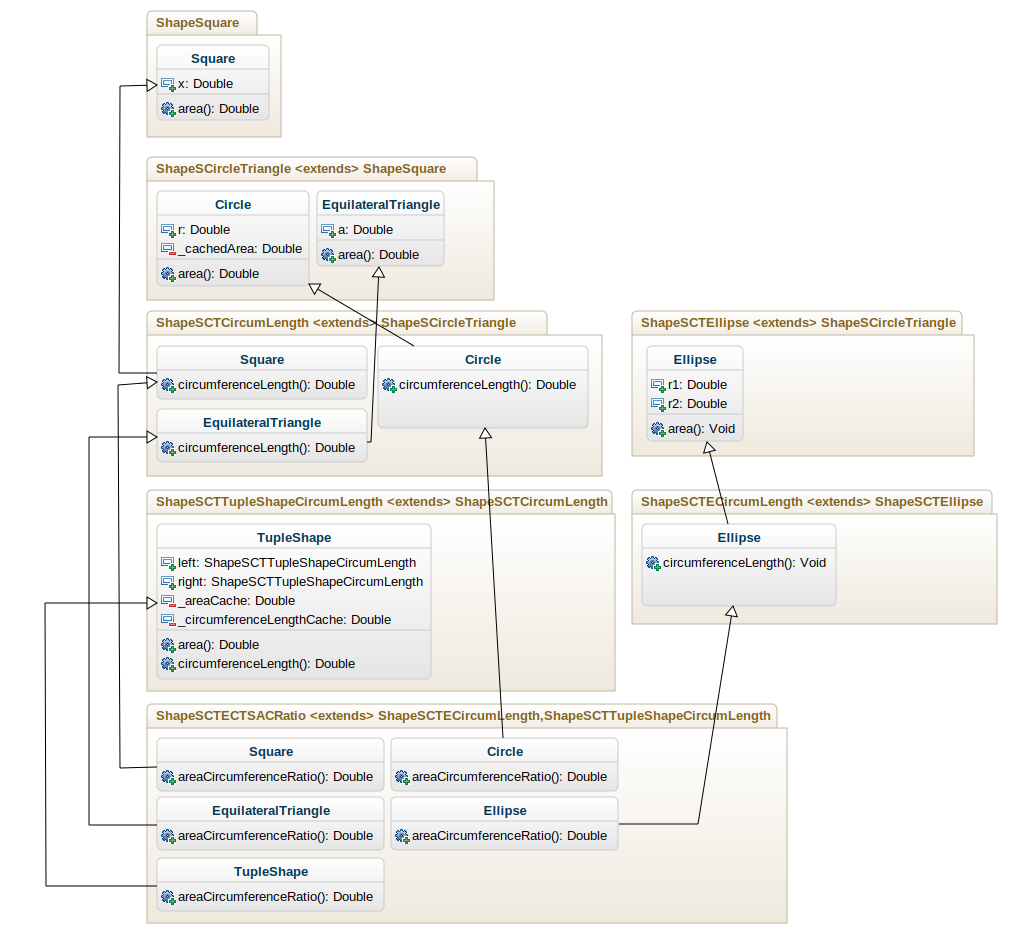
\includegraphics[width=330px,keepaspectratio=true]{Expression_problem-diag2.jpg}
\caption{Class Diagram of Use Case}
\end{figure}

\listoffigures

\chapter*{Acknowledgements}
I want to thank Tillmann Rendel for his outstanding technical and conceptual support with the whole paper. Also I want to thank Sebastian Erdweg for fixing the bugs I found and providing technical support in the implementation with SugarJ. Thanks also to all people that helped me with correcting this paper. Special thanks goes to Peter McAuley who spent much of his spare time with providing great feedback with corrections.

\begingroup
\renewcommand{\cleardoublepage}{}
\renewcommand{\clearpage}{}

\bibliographystyle{plain}

\bibliography{testFile} % no suffix

\endgroup
\end{document}

















